\section{Simulation}
\todo{rewrite and clean up}

\subsection{Data Generation}
Data is simulated from
\[
Y = \beta X + \varepsilon_Y
\]
where $X$ is generated by 
\[
X = \mu_{ZX}Z + \varepsilon_X
\]
with $Z \sim N(0,1)$. In order to test the models under different regimes, we utilise three different shock families for $\varepsilon_Y$: Normal ($\sim N(0,1)$), t ($\sim t(\nu)$), and centered Pareto ($\sim Pareto(\alpha)$). The base values are: $\beta = 1, \mu_{ZX}=1, \sigma^2_{ZX}=2.5, \sigma^2_{Z\varepsilon}=1, \rho=0.5, \delta=0.05,$ and $ n=2000$ unless stated otherwise. At this n, all strong instrument conditions hold.

\subsection{Competitor Estimator}
\label{sec:sim_catoni}

Besides the standard IV estimator of Section~\ref{sec:standard_iv}, we include Catoni's M-estimator of the mean \citep{catoni2012challenging} as a competitor. Alongside Median-of-Means, it is the other canonical sub-Gaussian mean estimator under the sole assumption of finite variance \citep{devroye2016sub}, which makes it the natural robust benchmark for the estimators of Sections~\ref{sec:rom}--\ref{sec:mor}.

For a sample $(V_i)_{i=1}^{n}$ with mean $\mu_V$ and variance $\sigma_V^2$, Catoni's estimator $\hat{\mu}_V^{\mathrm{Cat}}$ is the root of
\[
    \sum_{i=1}^{n} \psi\bigl(\alpha(V_i - \theta)\bigr) = 0,
    \qquad
    \psi(u) = \mathrm{sign}(u)\,\ln\!\left(1 + \abs{u} + \tfrac{u^2}{2}\right),
\]
where the bounded influence function $\psi$ replaces the identity implicit in the sample mean, so that no single observation can move the estimate by more than $O(1/\alpha)$. The tuning parameter $\alpha$ is chosen from the target confidence level and the noise scale as
\[
    \alpha = \sqrt{\frac{2\ln(2/\delta)}{n v \left(1 + \frac{2\ln(2/\delta)}{n - 2\ln(2/\delta)}\right)}},
\]
which, for any variance bound $v \geq \sigma_V^2$, yields a sub-Gaussian deviation guarantee at confidence level $1-\delta$ \citep{catoni2012challenging}. In the simulations $v$ is not treated as known: it is replaced by a preliminary Median-of-Means estimate of the variance, so that the tuning itself remains valid under heavy tails and the comparison does not favour Catoni through oracle knowledge of scale.

The IV analogue mirrors the Ratio-of-Medians construction: both cross-moments are estimated by Catoni's method and the ratio is taken,
\[
    \hat{\beta}_{\mathrm{Cat}} = \frac{\hat{\mu}_{ZY}^{\mathrm{Cat}}}{\hat{\mu}_{ZX}^{\mathrm{Cat}}},
\]
with the confidence budget split evenly across the two coordinates, i.e.\ each estimate is tuned at level $\delta/2$, matching the allocation used by the Ratio-of-Medians estimator in Theorem~\ref{thm:rom}. Since the root equation is strictly decreasing in $\theta$, each estimate is computed exactly by bisection.

\subsection{Simulation Results}
\label{ss:simulation_results}

\subsubsection{Cost of Robustness under Gaussian Errors}
\label{sss:e1}

\begin{figure}[htbp]
  \centering
  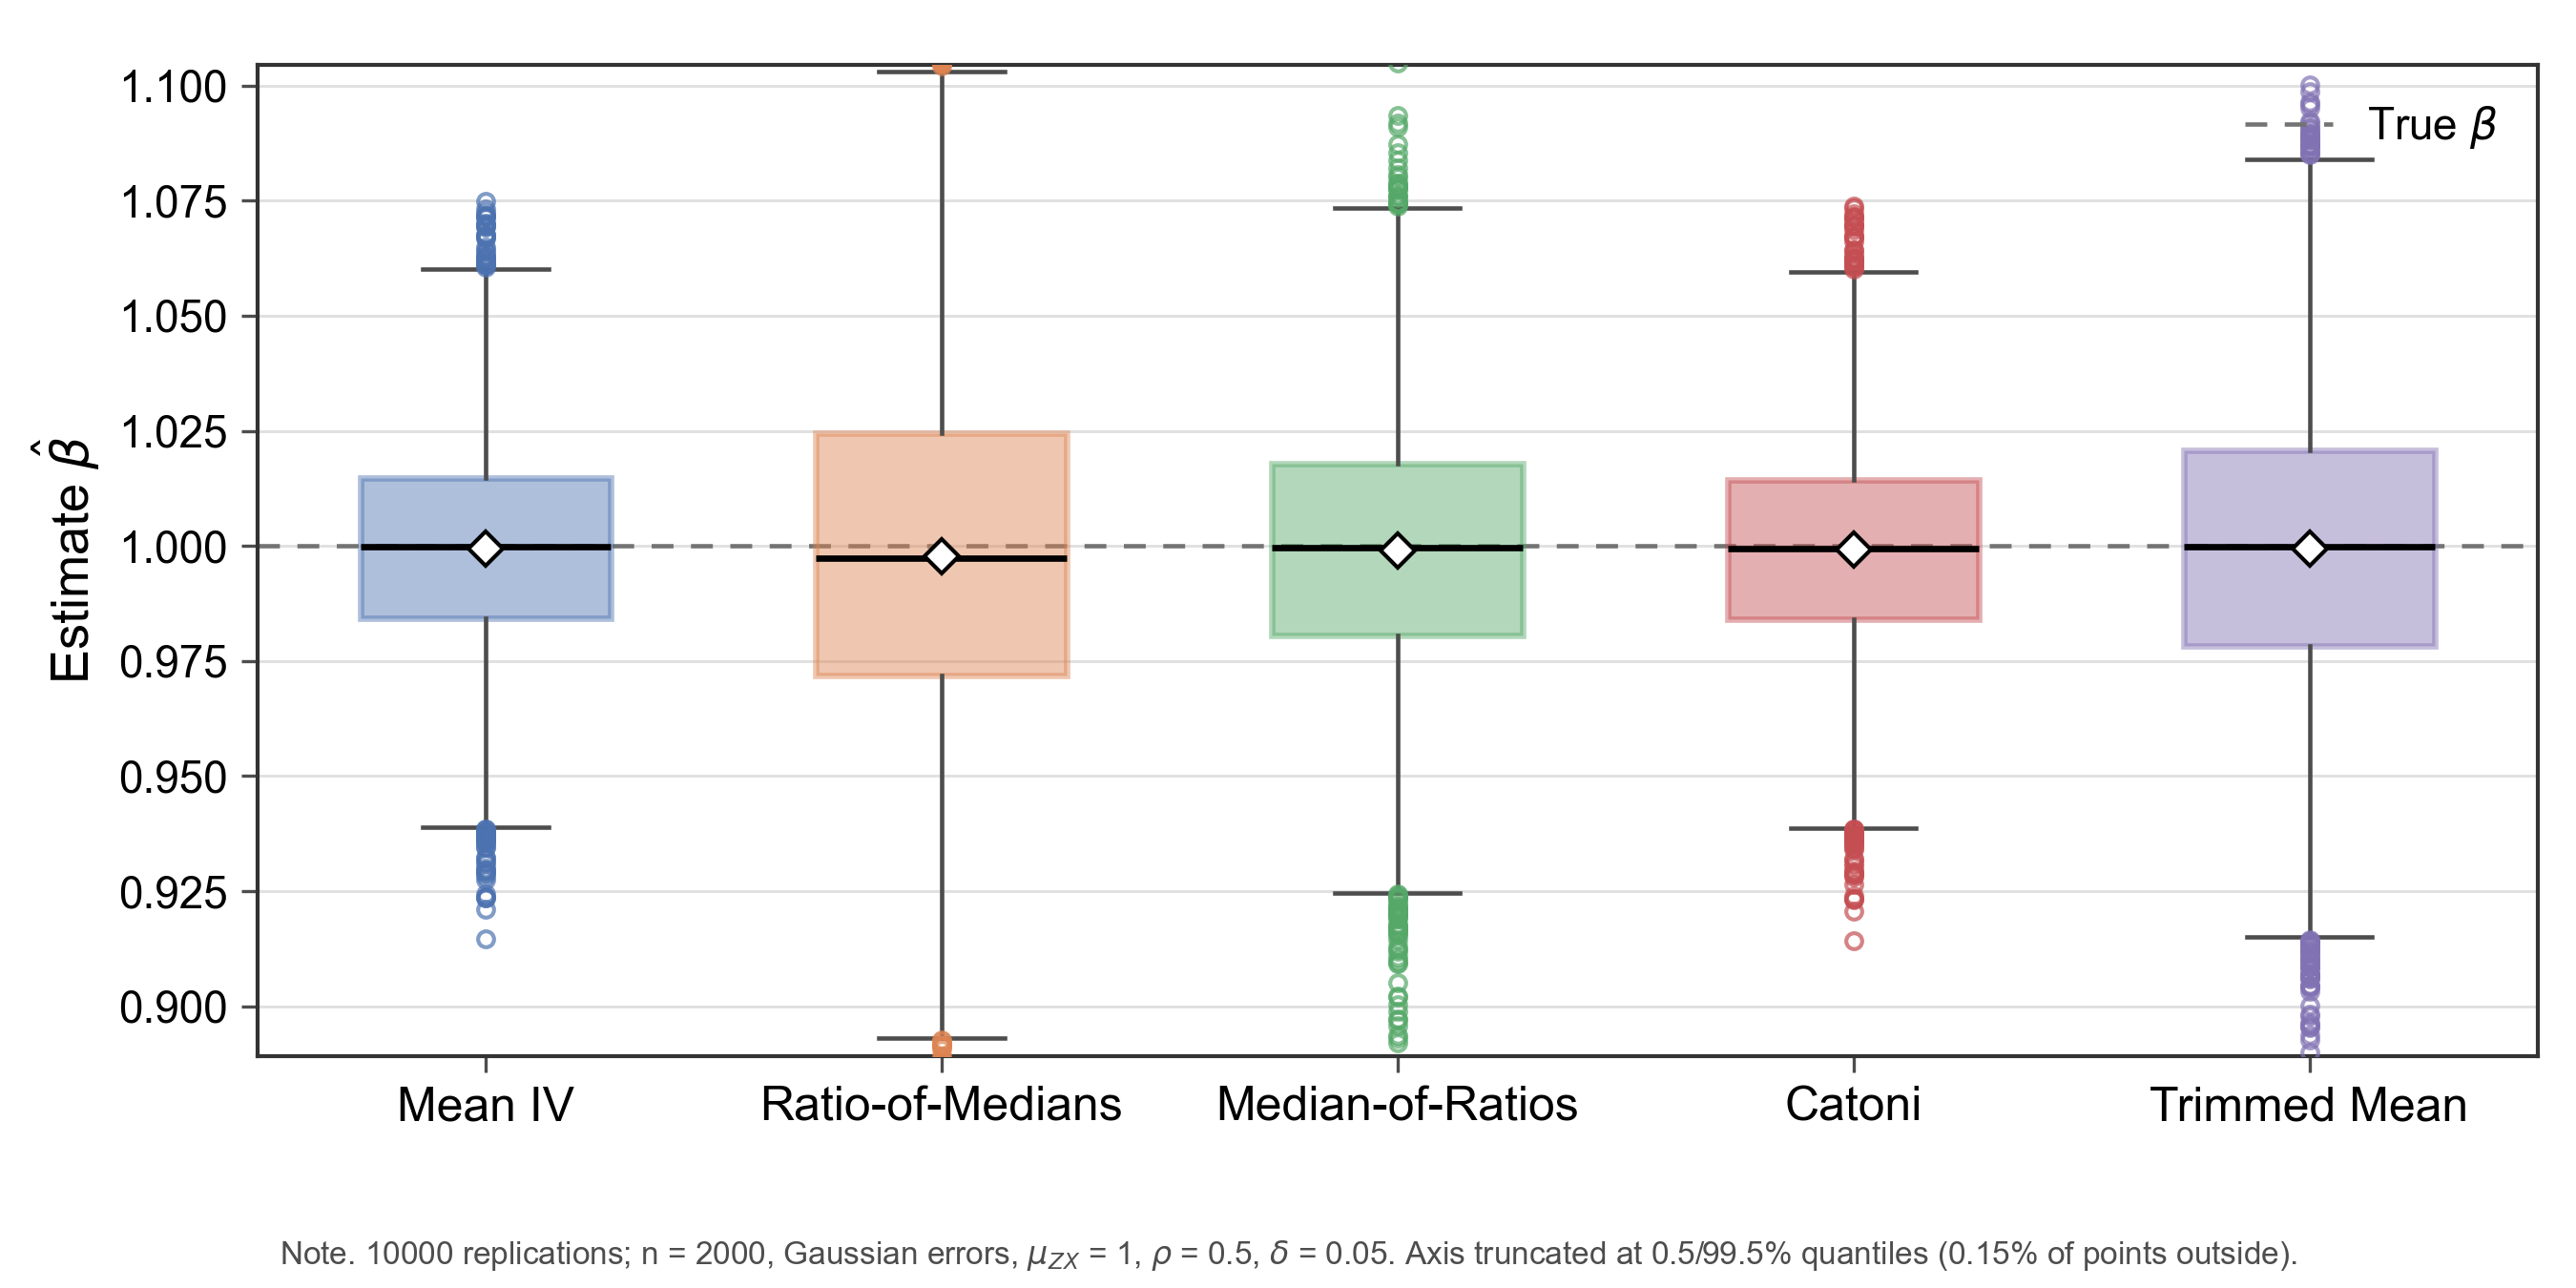
\includegraphics[width=0.8\textwidth]{images/graphs/e1_boxplot_gaussian.png}
  \caption{Boxplot showing the cost of robustness under Gaussian errors}
  \label{fig:e1_boxplot_gaussian}
\end{figure}

As can be seen in Figure~\ref{fig:e1_boxplot_gaussian}, all four estimators are unbiased, but their spreads differ. Mean IV and Catonig both have a standard deviation of 0.0224, MoR of 0.0274, and RoM 0.0396. These results are exactly as expected; under light tails, the sample mean is already the efficient estimator, so blocking and taking medians only throws information away. Catoni has equal results to the Mean IV because its influence funciton is nearly linear on well-behaved data. That it, the Catoni estimator is the mean until extreme observations appear.


\subsubsection{Benefit of Robustness under heavy tails}
\label{sss:e2}

\begin{figure}[htbp]
  \centering
  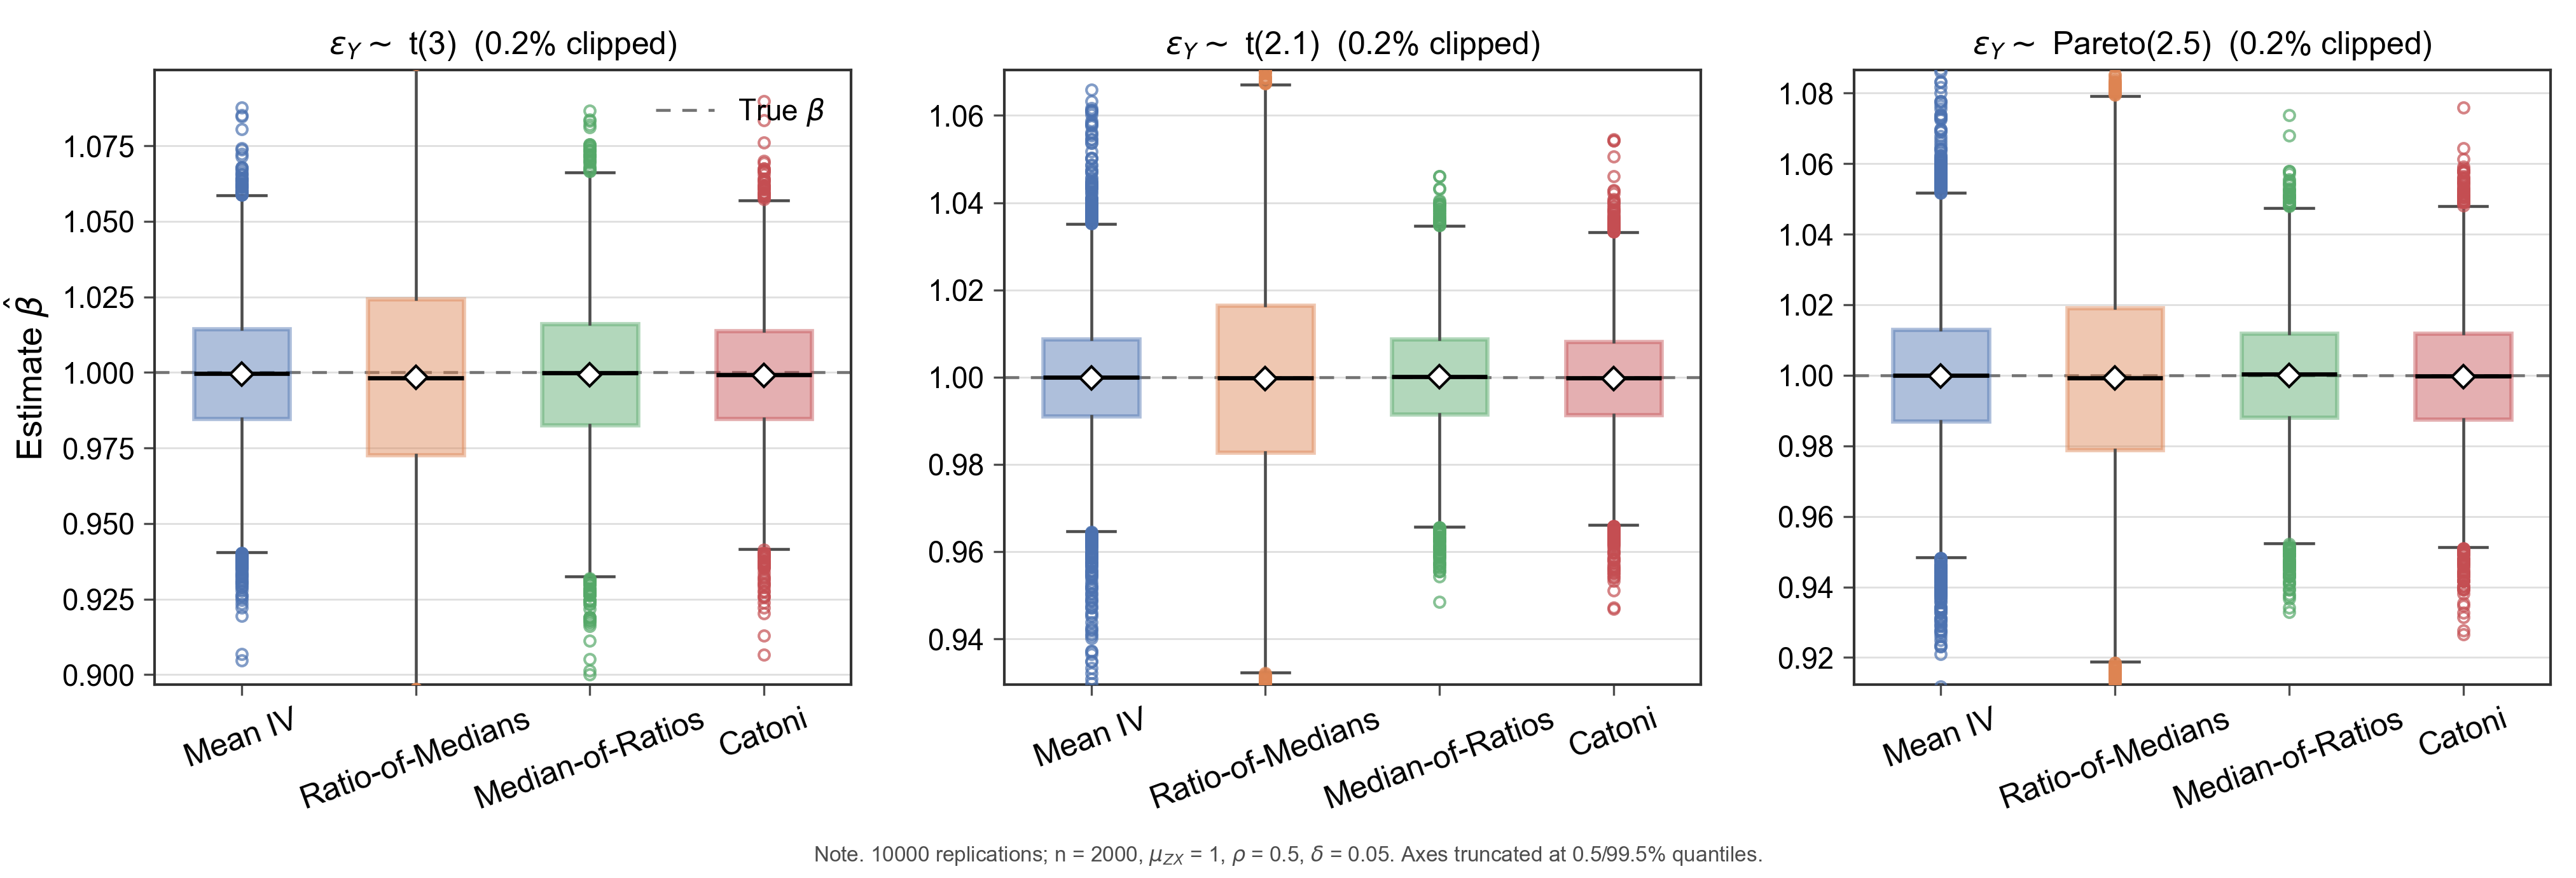
\includegraphics[width=0.8\textwidth]{images/graphs/e2_boxplot_heavytails.png}
  \caption{Boxplot showing the benefit of robustness under $t(3), t(2.1),$ and $Pareto(2.5)$ tails}
  \label{fig:e2_boxplot_heavytails}
\end{figure}

As per FIgure~\ref{fig:e2_boxplot_heavytails}, the benefit of MoM-type estimators becomes clear under $T(2.1)$ errors; the RMSE is 0.0128 for MoR and 0.0130 for Catoni against 0.0189 for Mean IV. The error quantile is 0.0341 under MoR and 0.0446 under Mean IV. RoM is clearly insufficient in all cases.

The IQR of the Mean IV and MoR estimators are very similar; the difference between the two is in the outliers, with MoR being much less susceptible to extreme values. This is expected, as MoM-type estimators do not promise variance bounds, but tail bounds, so the benefit lives in the tails. The Pareto panel shows no bias for any of the estimators, showing that all estimators can deal with asymmetric distributions.

Catoni and MoR shows very similar results but, visually, MoR seems to slightly improve on Catoni's tails, but this conclusion is only drawn from a visual inspection of the graph. Even if Both estimator yielded the same simulation results, the partsimony of the MoR estimator may make it more appealing if the data is known to be heavy tailed.


\subsubsection{$\delta$-dependence}
\label{sss:e2b}

\begin{figure}[htbp]
  \centering
  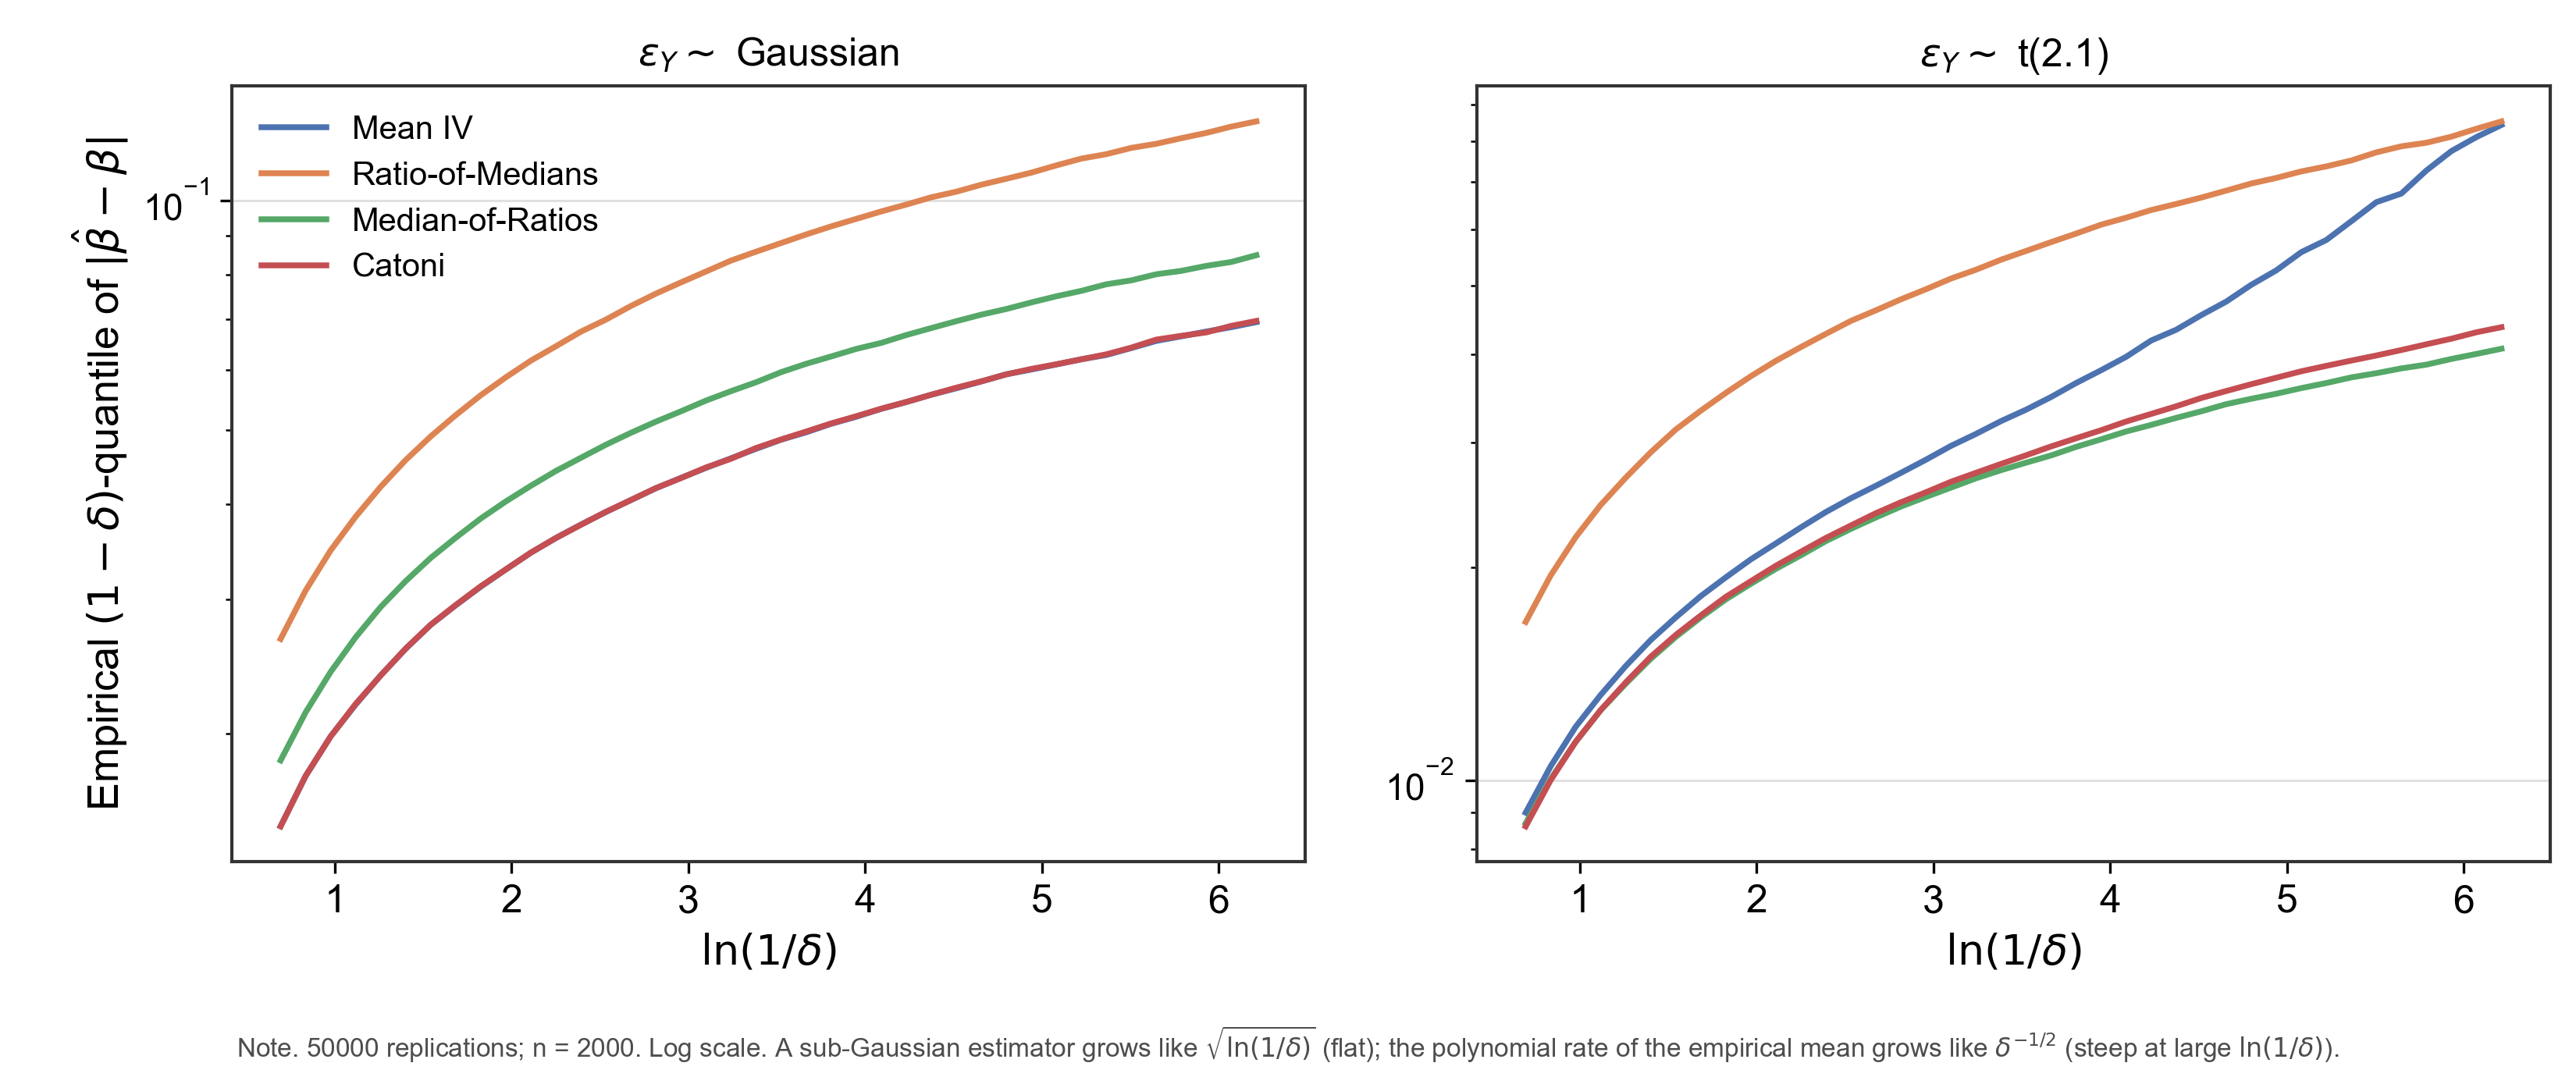
\includegraphics[width=0.8\textwidth]{images/graphs/e2b_deviation_quantiles.png}
  \caption{Graph showing the empirical $(1-\delta)$-quantile of $\abs{\hat{\beta} - \beta}$ against $\ln(1/\delta)$. Catoni and Mean IV have a near identical graph in the Normal regime}
  \label{fig:e2b_deviation_quantiles}
\end{figure}

Figure~\ref{fig:e2b_deviation_quantiles} shows that, for the Normal panel, All four curves are parallel and gently concave, meaning that every estimator is effectively sub-Gaussian, with Mean IV and Catonia sitting the lowest at every $\delta$. In the $t(2.1)$ regime we can see that the Mean IV estimator becomes convex at around $\ln(1/\delta) = 4$ which, as stated by Remark~\ref{rem:iv_polynomial}, is unavoidable. The more confidence is demanded, the more MoM wins when compared against Mean IV. The slight benefit that MoR showed against Catoni in Section~\ref{sss:e2} is also visible here, with MoR having a slightly smaller quantile than Catoni as $\delta$ increases.


\subsubsection{Instrument Strength Conditions}
\label{sss:e3}

\begin{figure}[htbp]
  \centering
  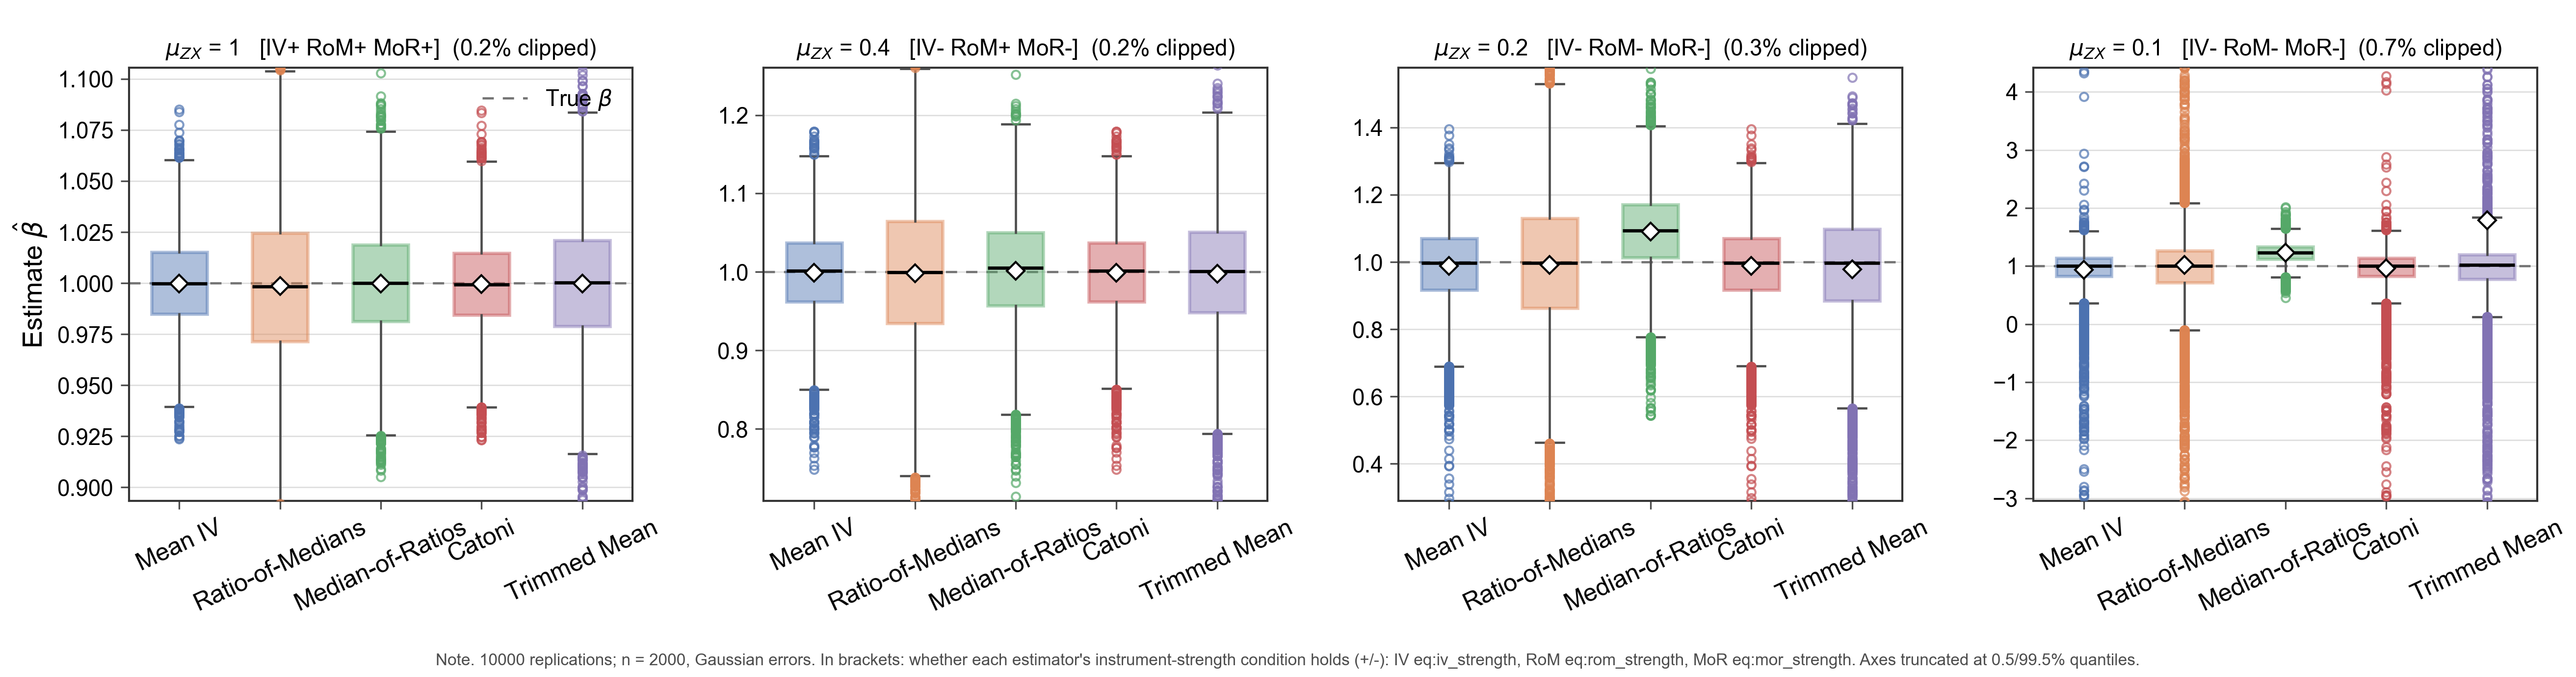
\includegraphics[width=0.8\textwidth]{images/graphs/e3_boxplot_strength.png}
  \caption{Boxplot showing the effect of weaker instrument strength conditions with a sweeping $\mu_ZX$}
  \label{fig:e3_boxplot_strength}
\end{figure}

Figure~\ref{fig:e3_boxplot_strength} shows that, at $\mu_{ZX} = 0.4$, where MoM conditions fail but IV holds, every estimator is still centered, but Mean IV and Catoni are the tightest. As the instrument strength condition weakens, IV and Catoni stay mean centered, but produce terrible estimates, with a standard deviation of 2.5 and minimum and maximum values in the hundreds. MoR, though, remains stable, albeit highly biased, with a mean estimate of 1.23. On RMSE, MoR is the best fit here, with a value of 0.28, against 2.5 of Mean IV and 2.8 of Catoni. The RoM estimator performs worse on all cases. Under weak instruments, IV, RoM, and Catoni fail by variance explosion; and MoR fails by bias.

\subsubsection{Empirical Size}
\label{sss:i1}

\begin{figure}[htbp]
  \centering
  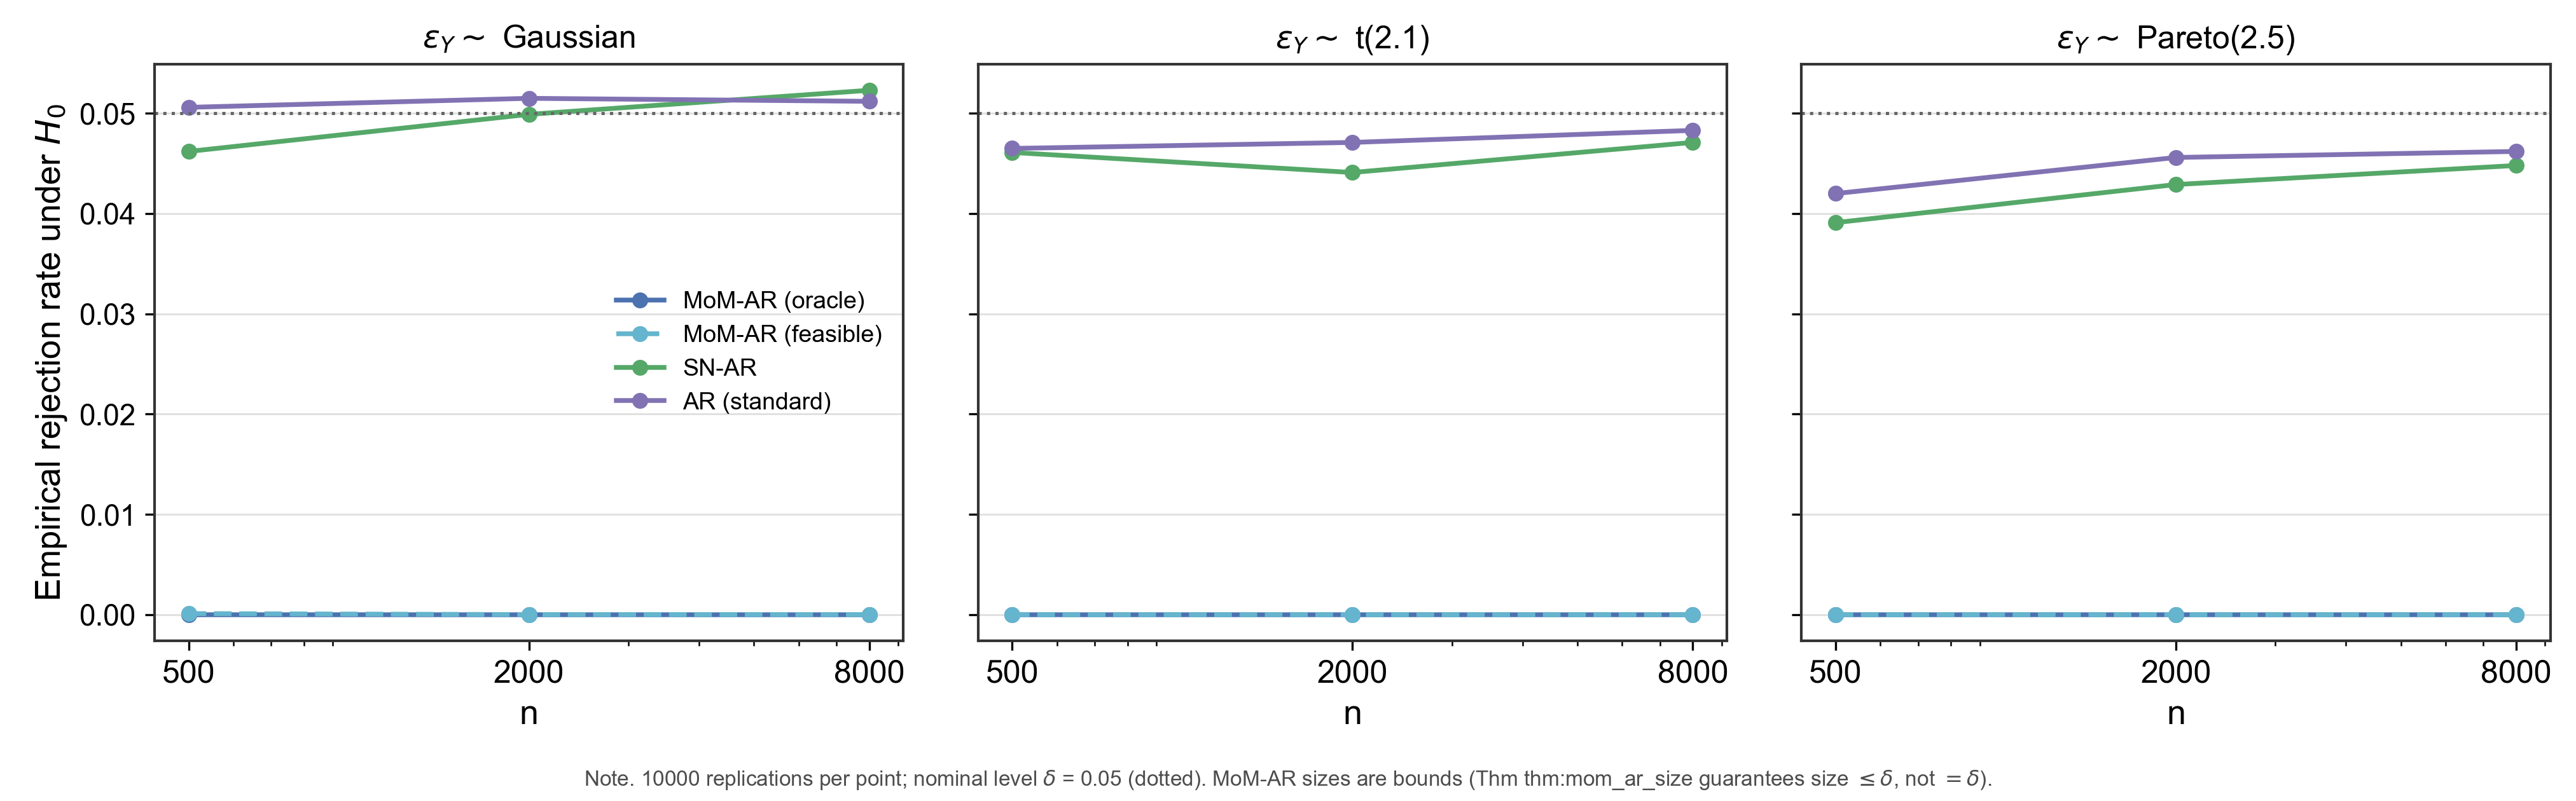
\includegraphics[width=0.8\textwidth]{images/graphs/i1_size.png}
  \caption{Plot of the size of all tests}
  \label{fig:i1_size}
\end{figure}

Figure~\ref{fig:i1_size} shows that, at the true $\beta$, botht eh oracleand feasible MoM-AR test teject in at most 0.01\% of 10,000 replications in every designe, against the nominal 5\%. The finite sample size bound of \ref{thm:mom_ar_size} holds and is very conservative; the oracle threshold $\tau_n$ is 7.9 times the actual standard deviation of the statistic under $H_0$ in the Gaussian design at $n=2000$, and 16.7 times under $t(2.1)$; it is built from Chebyschev and Hoeffding distribution agnostic worst case scenarios, so it is fixed by $\sigma_{Z\varepsilon}$ alone and cannot adapt to the tails. The feasible threshold, rebuilt from a robust scale estimate, instead stays between 7.0 and 7.3 times that standard deviation in every design and at every sample size.

Comparing the AR tests against each other, both are close enough to the nominal 5\% size value, though as the distirbutions get heavier tails ($t(2.1)$ and $Pareto(2.5)$), they bocem slightly more conservative. It is worth noting that the self-normalised AR test is consistently slightly more conservative than the standard AR test.

\subsubsection{Power of the Four Tests}
\label{sss:i2}

\begin{figure}[htbp]
  \centering
  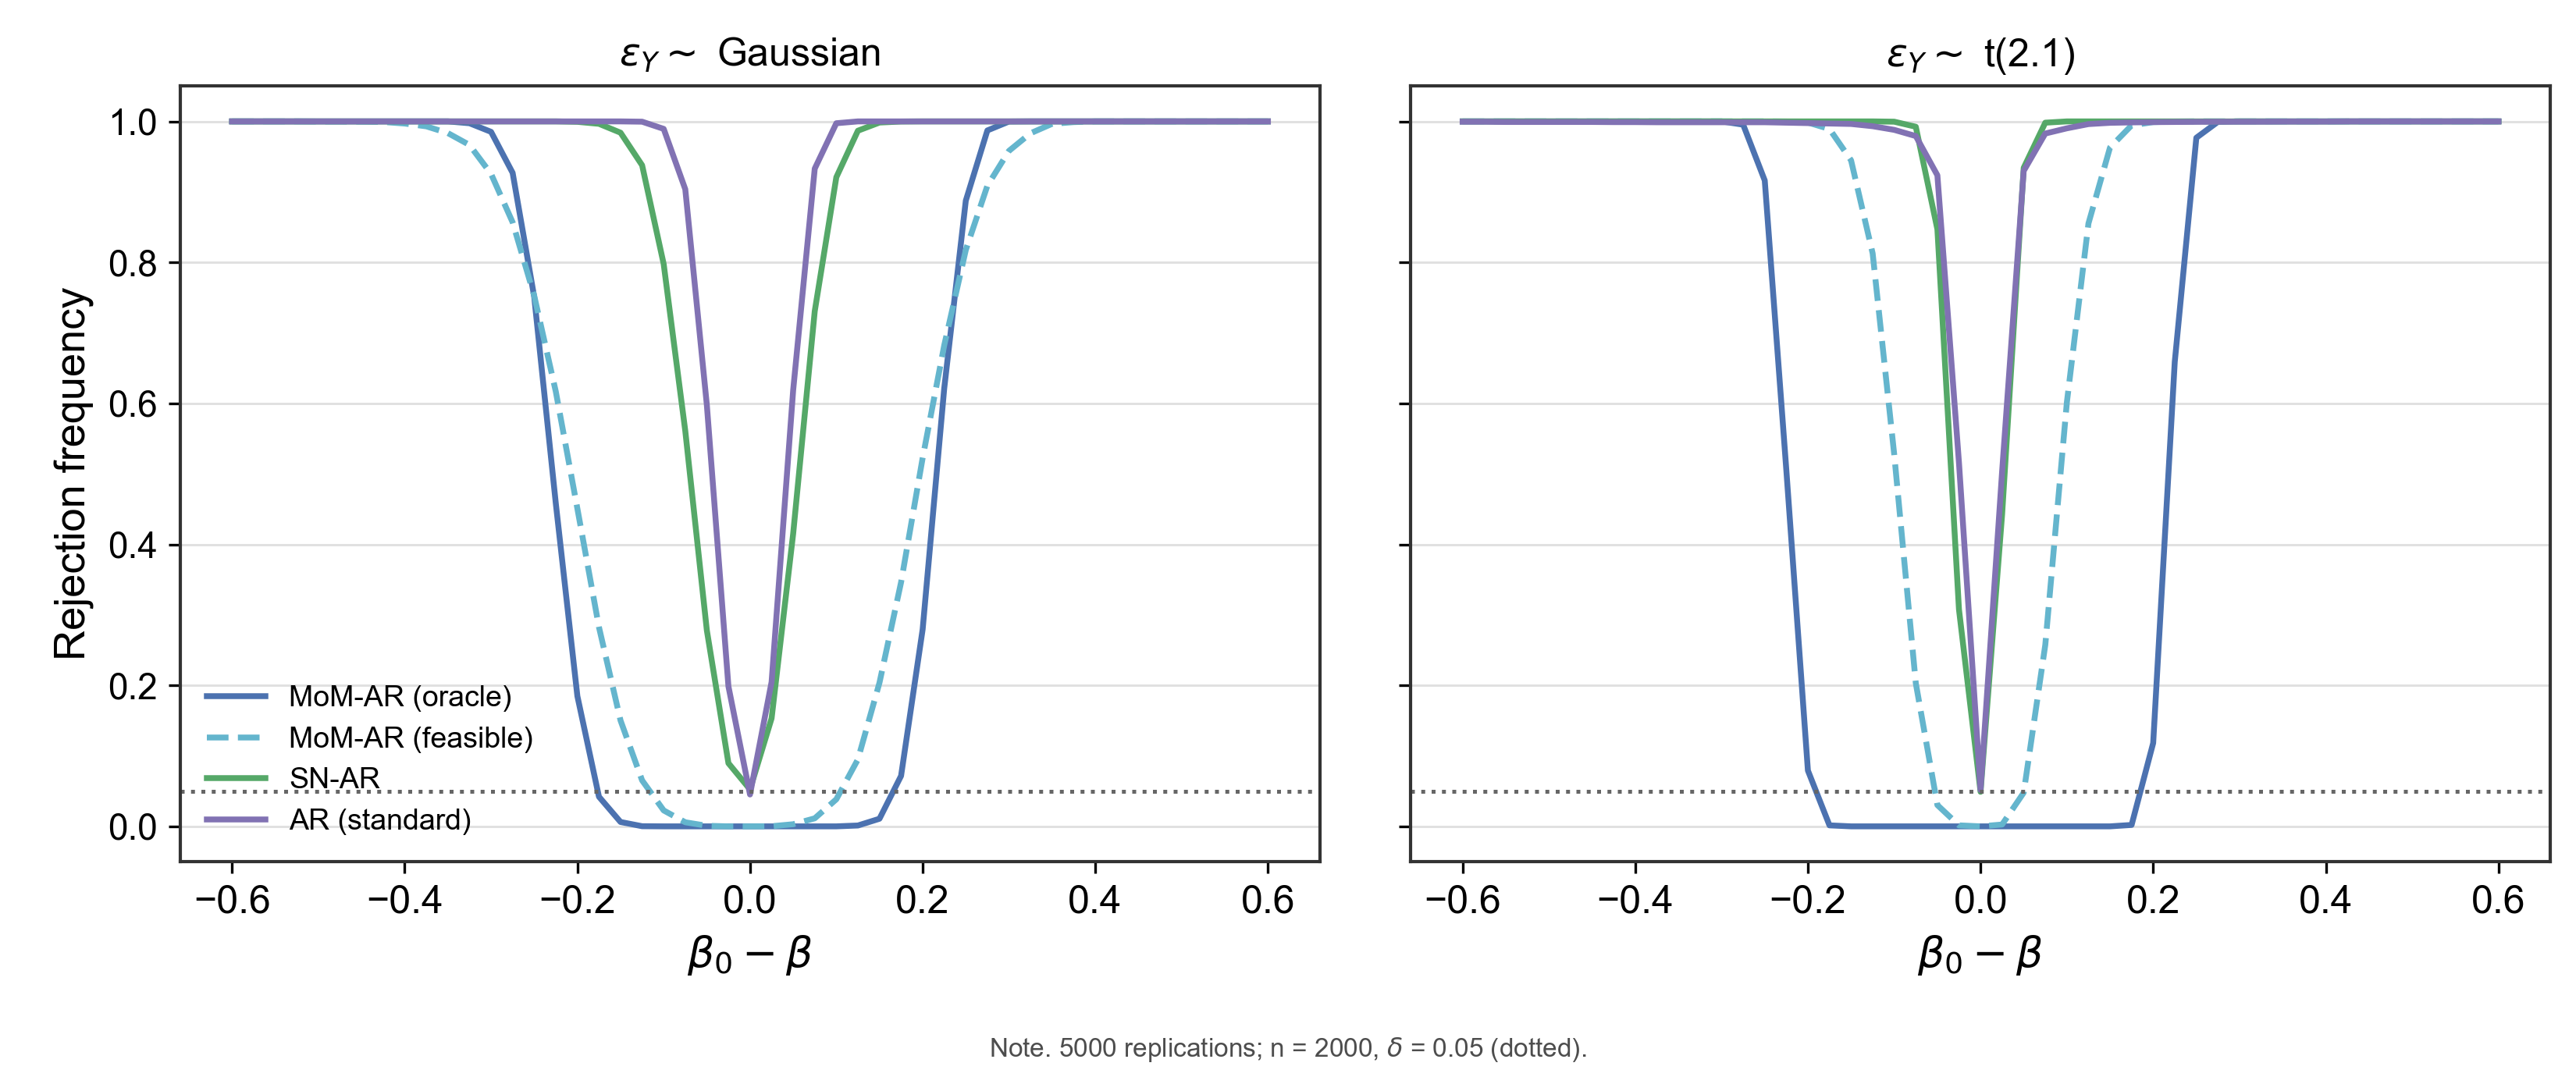
\includegraphics[width=0.8\textwidth]{images/graphs/i2_power.png}
  \caption{Power curves of all tests}
  \label{fig:i2_power}
\end{figure}

Figure~\ref{fig:i2_power} show that the MoM-AR acceptance regions are less powerful than the AR based tests, with the feasible version being slightly more powerful than the oracle version in the Normal setting. In the heavy tail setting, the feasible MoM-AR test is much more powerful. THis is due to the MAD-based scale estimate setting $\hat{\sigma}^{MAD}_{Z\varepsilon}$ below the true $\sigma_{Z\varepsilon}$. This is not a result that is expected and is a lucky cancellation due to the DGP, not a guarantee. The standard AR test is more powerful than the self-normalised AR test in the Normal setting, though this benefit decreases as tails become larger, as can be seen in the $t(2.1)$ case, where the due are nearly indistinguishable. If the finite-sample guarantee is needed, one has to pay in power, though, as can be seen by comparing the self-normalised to the standard AR, the cost is not that high.

\subsubsection{Partition Randomness}
\label{sss:ps}

\begin{figure}[htbp]
  \centering
  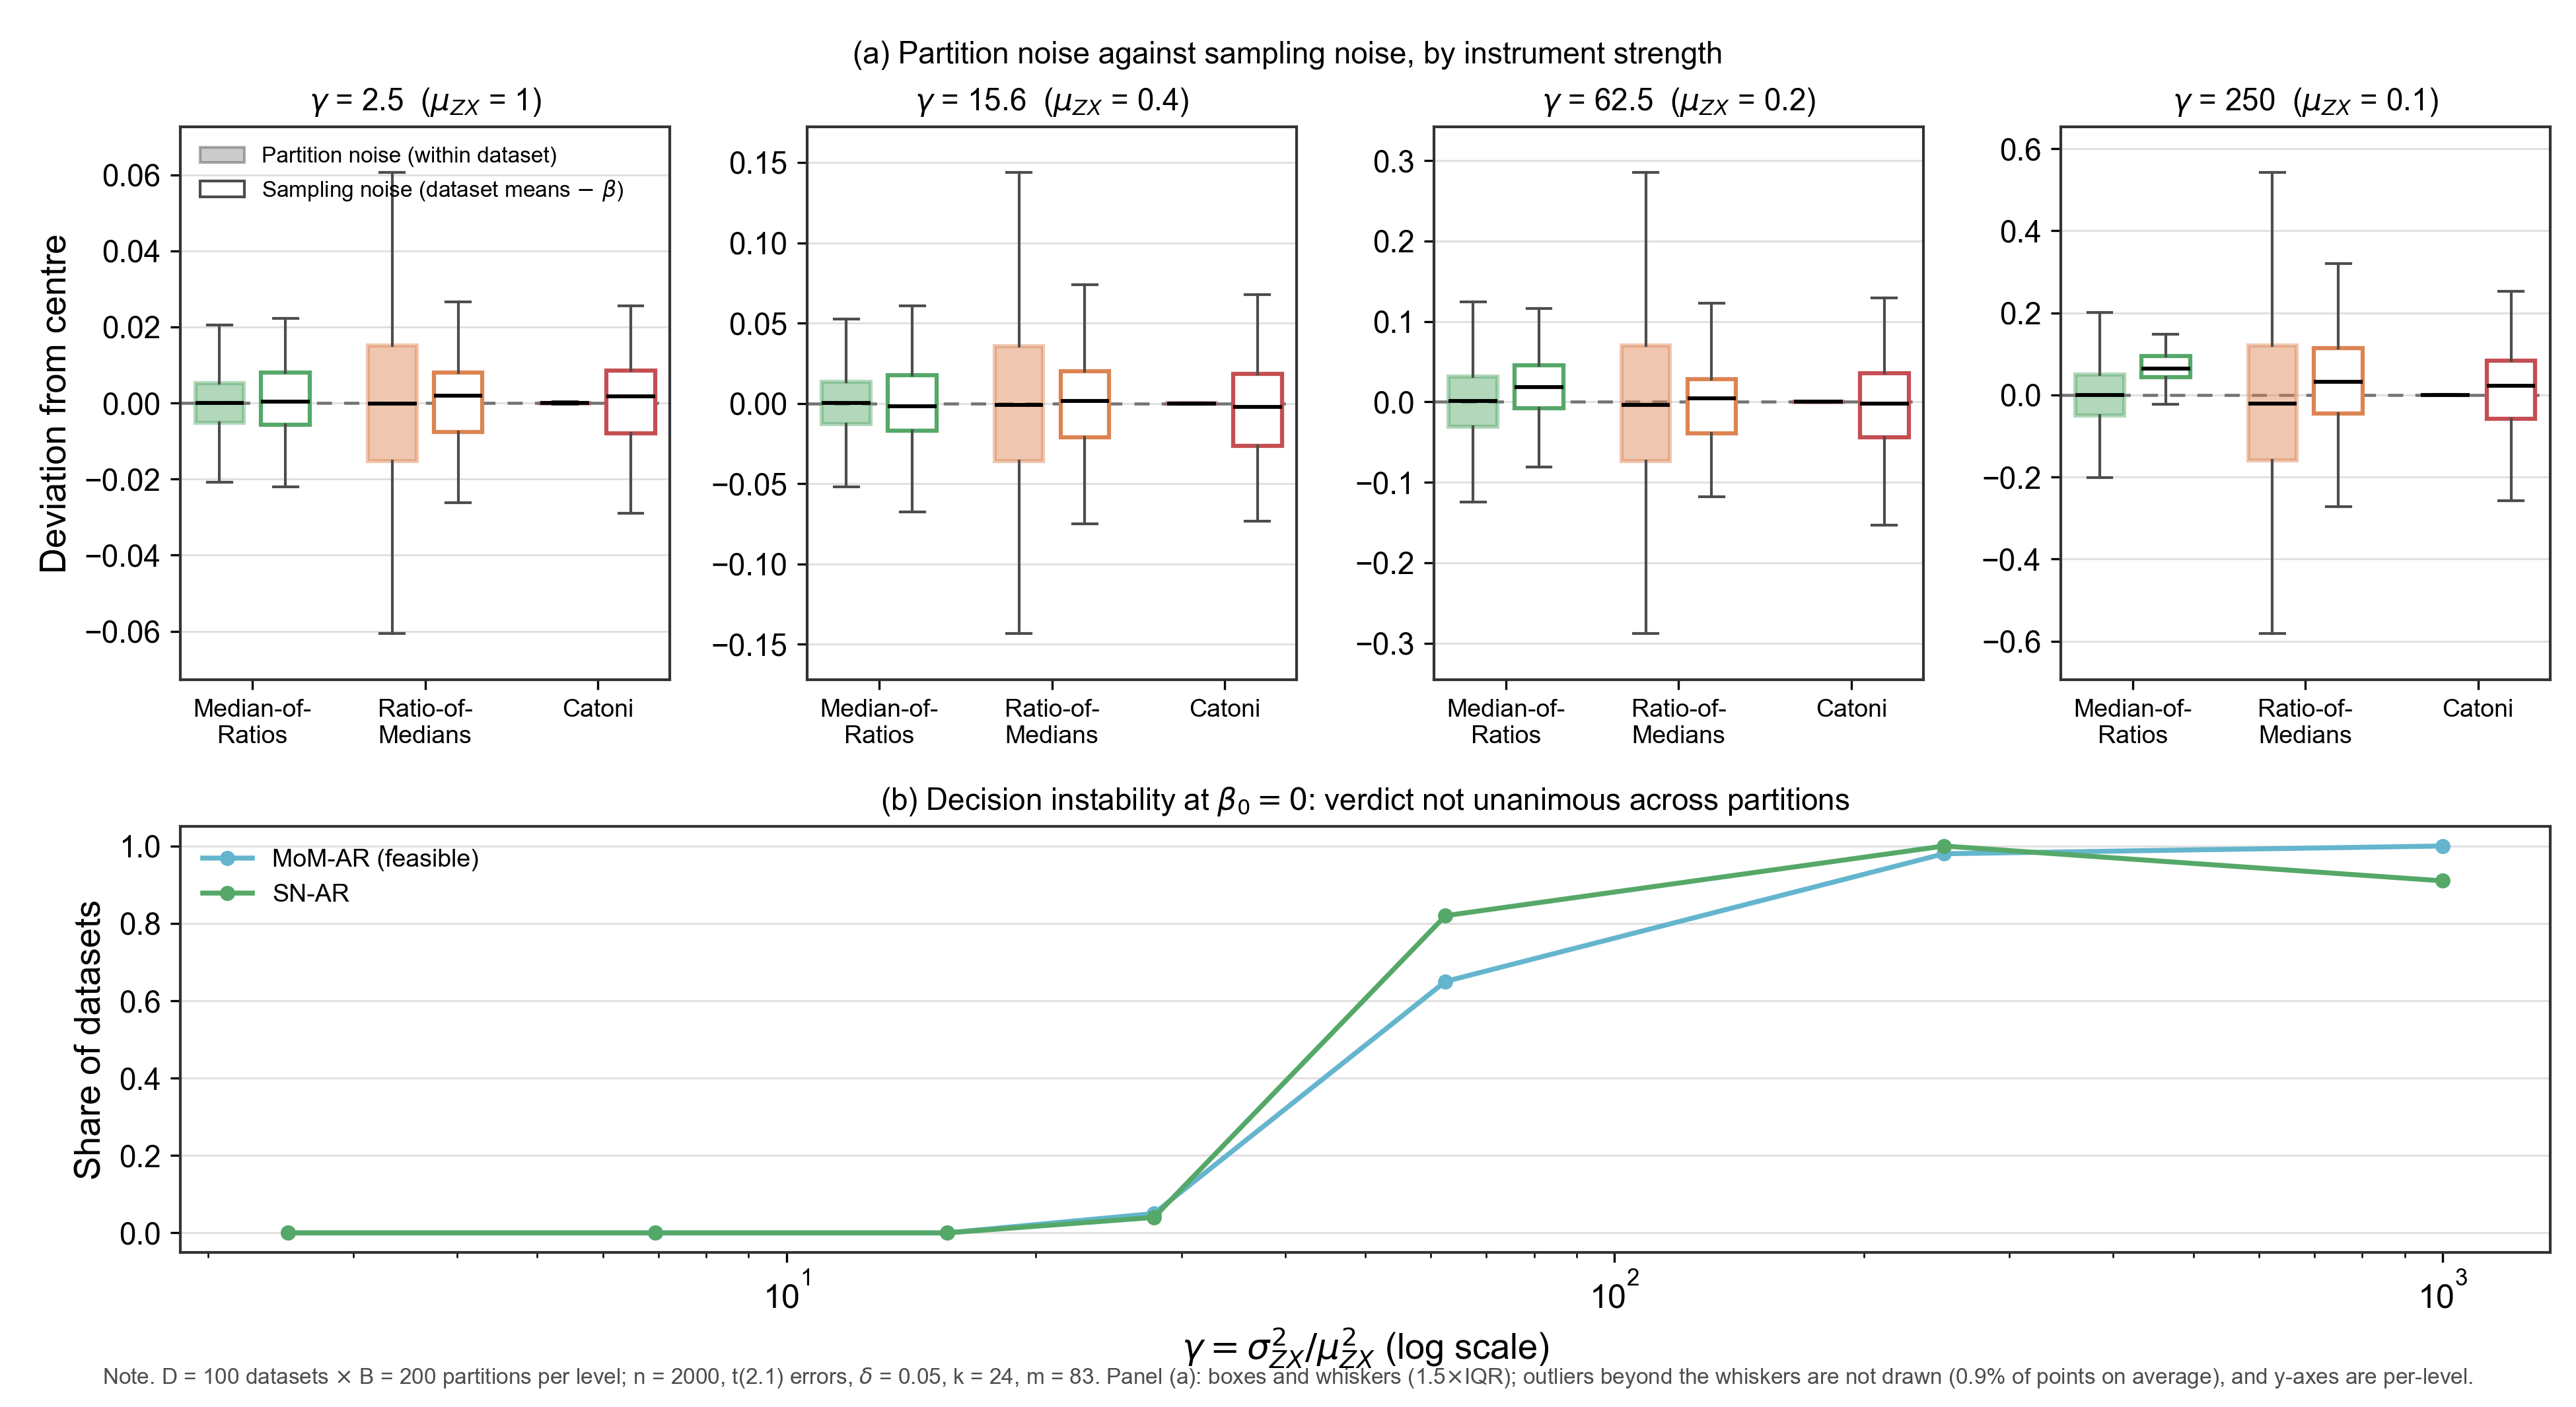
\includegraphics[width=\textwidth]{images/graphs/ps_partition_randomness.png}
  \caption{Partition noise against sampling noise, and the share of datasets whose test verdict at $\beta_0 = 0$ depends on the partition, against instrument strength $\gamma = \sigma^2_{ZX}/\mu_{ZX}^2$}
  \label{fig:ps_partition_randomness}
\end{figure}

Every estimator of Sections~\ref{sec:rom}--\ref{sec:mor} splits the sample into blocks, and on real data that split has to be randomised, since the observations do not arrive in a random order. The estimate therefore depends on the partition draw as well as on the data. Figure~\ref{fig:ps_partition_randomness} separates the two. For each instrument strength, $D = 100$ datasets are drawn and each is partitioned $B = 200$ times. Panel~(a) plots the deviation of every estimate from its own dataset's average across partitions (filled boxes, which isolate the partition), against the dataset averages centred at the true $\beta$ (hollow boxes, which isolate the data).

The partition is not a negligible source of noise even where the theory is comfortable. At $\gamma = 2.5$, where all strength conditions hold, the partition accounts for 34\% of the total variance of the Median-of-Ratios estimator and for 78\% of that of Ratio-of-Medians; in interquartile terms the Ratio-of-Medians partition box is roughly twice as wide as its sampling box. Catoni's estimator is effectively partition-free, as the blocking enters it only through the variance pre-estimate. As the instrument weakens both block estimators deteriorate, and the deterioration is mostly in the partition: the Median-of-Ratios share rises to 0.93 at $\gamma = 1000$, so that at that point the reported number is more a function of the seed than of the sample.

Panel~(b) asks what this costs a conclusion rather than an estimate. It reports the share of datasets on which the verdict at $\beta_0 = 0$ is \emph{not} unanimous across the 200 partitions, that is, on which rejecting the null depends on the seed. Up to $\gamma \approx 16$ the verdict is unanimous on every dataset, so the partition is inferentially irrelevant. Instability then rises steeply, to 65\% of datasets for the feasible MoM-AR test and 82\% for the self-normalised test at $\gamma = 62.5$, and to essentially every dataset by $\gamma = 250$. The two tests behave alike, so this is a property of the blocking rather than of the threshold.

\begin{figure}[htbp]
  \centering
  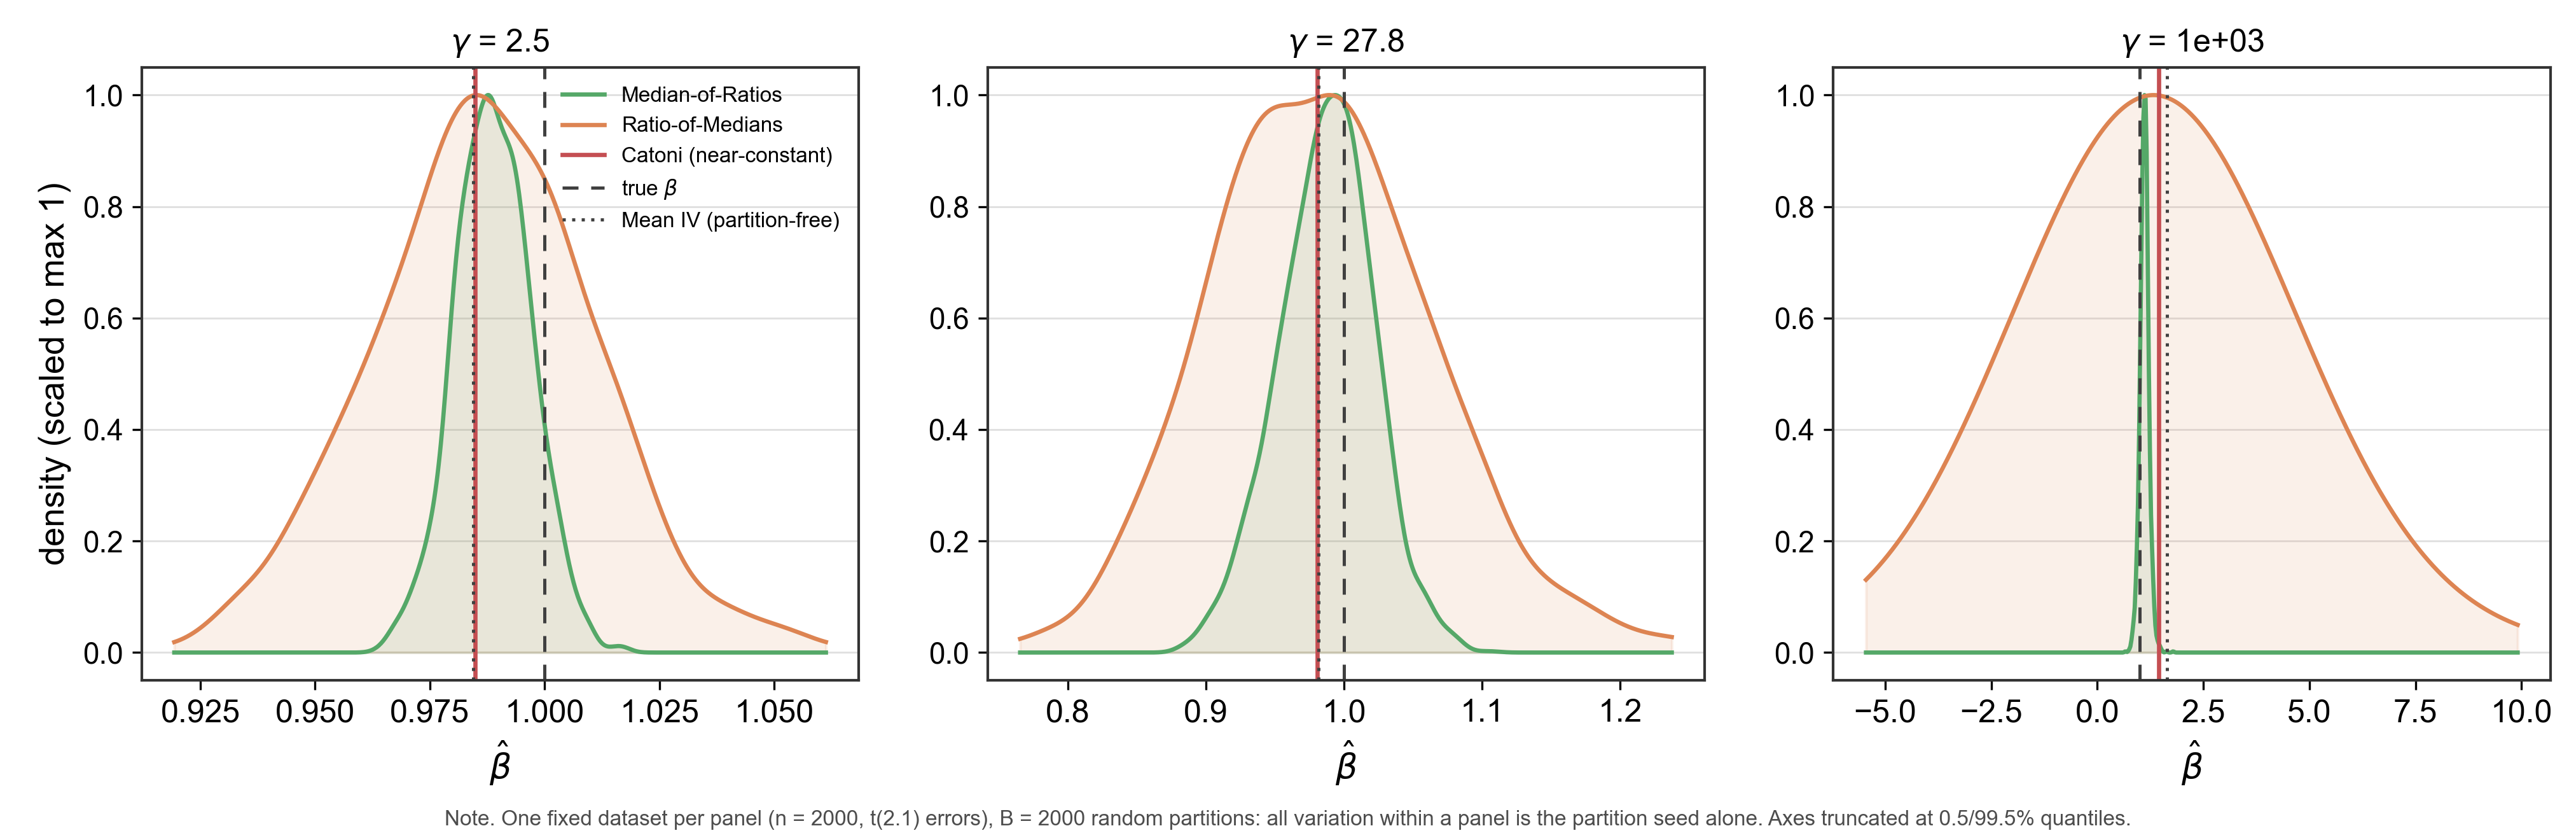
\includegraphics[width=\textwidth]{images/graphs/ps_partition_spotlight.png}
  \caption{Estimator distributions over random partitions of a single fixed dataset, at three instrument strength levels}
  \label{fig:ps_partition_spotlight}
\end{figure}

Figure~\ref{fig:ps_partition_spotlight} shows the same phenomenon from the position of a researcher holding one data set. Each panel fixes a single sample and redraws the partition 2,000 times, so all of the spread displayed is the seed alone; the partition-free Mean IV estimate is marked for reference. Under a strong instrument the two block estimators concentrate near it, with Ratio-of-Medians already visibly the wider of the two. At $\gamma = 1000$ the contrast is stark: Ratio-of-Medians ranges over roughly $[-5, 10]$ on a single data set, while Median-of-Ratios remains a narrow spike, displaced from $\beta$ but stable. This is the same division of failure modes seen in Section~\ref{sss:e3}, and it appears here without any resampling of the data at all.
